% Mutation-adequacy subsection.

\subsection{Mutation Adequacy}
\label{sec:mutation-adequacy}

\paragraph{Setup.}
Six $(\mathrm{SUT, format})$ pairs span four parser languages.
Mutation engines are PIT~\citep{coles2016pit} for htsjdk,
mutmut~\citep{mutmut2024} for vcfpy and biopython,
cargo-mutants~\citep{cargomutants2024} for noodles, and a DIY
mull-style \textsc{aor}/\textsc{ror}/\textsc{lor} operator
set~\citep{denisov2018mull,just2014mutants} for seqan3. The kill
predicate is a parse-success flip, canonical-JSON divergence,
or crash-class flip, scored as
$\mathit{killed}/\mathit{reachable}$~\citep{coles2016pit,papadakis2019mutation}
identically between \biotest{} and each baseline. We run
$n{=}10$ replicates on the four close-margin pairs (htsjdk/VCF,
htsjdk/SAM, vcfpy/VCF, noodles/VCF) and $n{=}4$ on biopython and
seqan3, where samples are deterministic. Baselines and \biotest{} share the Tier-1+2 spec-example seed
foundation. \biotest{} additionally carries its Phase-D
synthetic outputs and augmentation tier as part of its deployed
pipeline. We report end-to-end deployed performance rather than
a synthetic seed-only ablation.

% Mutation-adequacy radar -- single-column.
%
% Design:
%   - hexagonal grid (concentric hexagons + 6 radial spokes)
%   - no vertex markers, no numerical value labels
%   - tools that cover >= 2 SUTs are drawn as filled polygons
%     (BioTest 6 axes, Pure-Random 6 axes, Jazzer triangle on
%      htsjdk-VCF + htsjdk-SAM, Atheris degenerate line on
%      vcfpy + biopython which are 180 deg apart)
%   - single-SUT tools (cargo-fuzz, libFuzzer, AFL++) are drawn
%     as a single coloured dot at the value position on their
%     applicable axis
%   - all polygon outlines are kept thin so the shaded areas
%     dominate over outline
%
% Width is sized for IEEEtran's single column (~88mm).

\begin{figure}[!t]
\centering
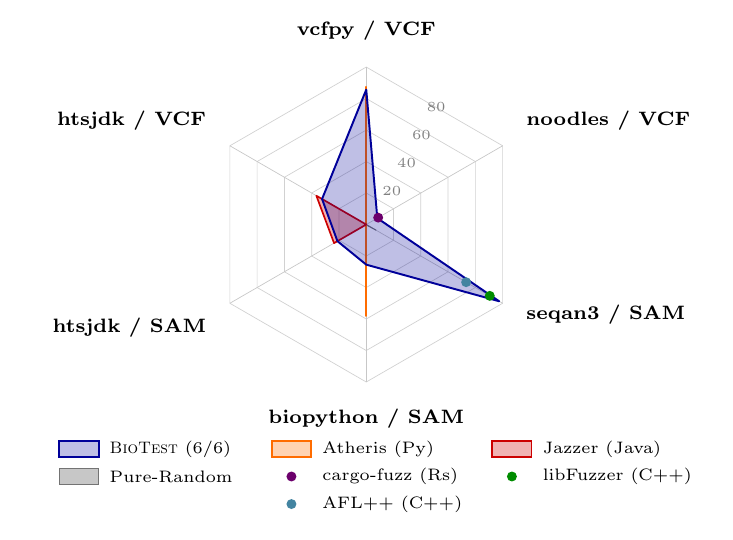
\begin{tikzpicture}

\colorlet{btblue}{blue!60!black}
\colorlet{atherisclr}{orange!85!red}
\colorlet{jazzerclr}{red!80!black}
\colorlet{cargoclr}{violet!85!black}
\colorlet{libfclr}{green!55!black}
\colorlet{aflclr}{cyan!60!black}
\colorlet{prclr}{black!55}

\pgfmathsetmacro{\R}{2.0}
\useasboundingbox (-4.3,-3.65) rectangle (4.3,2.50);

% ---- (1) hexagonal grid + spokes --------------------------------
\foreach \pct in {20,40,60,80,100}{%
  \draw[draw=black!18, line width=0.25pt, line join=round]
        (90:{\R*\pct/100}) -- (30:{\R*\pct/100})
     -- (-30:{\R*\pct/100}) -- (-90:{\R*\pct/100})
     -- (-150:{\R*\pct/100}) -- (150:{\R*\pct/100}) -- cycle;
}
\foreach \pct in {20,40,60,80}{%
  \node[font=\fontsize{5}{5.5}\selectfont, text=black!50,
        anchor=south west, inner sep=0.3pt]
        at (62:{\R*\pct/100}) {\pct};
}
\foreach \ang in {90,30,-30,-90,-150,150}{%
  \draw[draw=black!22, line width=0.25pt] (0,0) -- (\ang:\R);
}

% ---- (2) Pure-Random hexagonal floor (multi-SUT, shaded) -------
\filldraw[fill=prclr, fill opacity=0.40,
          draw=prclr, line width=0.35pt, line join=round]
   (90:{\R*0.0089}) -- (30:0) -- (-30:{\R*0.0719})
-- (-90:{\R*0.0024}) -- (-150:{\R*0.0120}) -- (150:0) -- cycle;

% ---- (3) Atheris (multi-SUT but two collinear axes; the polygon
%          is geometrically degenerate and renders as a thin
%          shaded line through the origin) -----------------------
\filldraw[fill=atherisclr, fill opacity=0.30,
          draw=atherisclr, line width=0.7pt, line join=round]
   (90:{\R*0.8737}) -- (30:0) -- (-30:0)
-- (-90:{\R*0.5800}) -- (-150:0) -- (150:0) -- cycle;

% ---- (4) Jazzer (multi-SUT, filled triangle in the left half) --
\filldraw[fill=jazzerclr, fill opacity=0.30,
          draw=jazzerclr, line width=0.6pt, line join=round]
   (90:0) -- (30:0) -- (-30:0)
-- (-90:0) -- (-150:{\R*0.2361}) -- (150:{\R*0.3659}) -- cycle;

% ---- (5) BioTest hexagon (top layer, dominant area) ------------
\filldraw[fill=btblue, fill opacity=0.25,
          draw=btblue, line width=0.7pt, line join=round]
   (90:{\R*0.8566}) -- (30:{\R*0.0810}) -- (-30:{\R*0.9744})
-- (-90:{\R*0.2548}) -- (-150:{\R*0.2114}) -- (150:{\R*0.3240})
-- cycle;

% ---- (6) Single-SUT tools as dots ------------------------------
\fill[cargoclr] (30:{\R*0.0874}) circle (1.8pt);
\fill[libfclr]  (-30:{\R*0.9057}) circle (1.8pt);
\fill[aflclr]   (-30:{\R*0.7322}) circle (1.8pt);

% ---- (7) per-axis SUT/format labels ----------------------------
\node[anchor=south, inner sep=1pt,
      font=\fontsize{7.5}{7.5}\selectfont\bfseries]
      at (90:{\R + 0.30}) {vcfpy / VCF};
\node[anchor=south west, inner sep=1pt,
      font=\fontsize{7.5}{7.5}\selectfont\bfseries]
      at (30:{\R + 0.30}) {noodles / VCF};
\node[anchor=west, inner sep=1pt,
      font=\fontsize{7.5}{7.5}\selectfont\bfseries]
      at (-30:{\R + 0.30}) {seqan3 / SAM};
\node[anchor=north, inner sep=1pt,
      font=\fontsize{7.5}{7.5}\selectfont\bfseries]
      at (-90:{\R + 0.30}) {biopython / SAM};
\node[anchor=north east, inner sep=1pt,
      font=\fontsize{7.5}{7.5}\selectfont\bfseries]
      at (-150:{\R + 0.30}) {htsjdk / SAM};
\node[anchor=south east, inner sep=1pt,
      font=\fontsize{7.5}{7.5}\selectfont\bfseries]
      at (150:{\R + 0.30}) {htsjdk / VCF};

% ---- (8) compact 3-row x 3-col legend below the radar ---------
\begin{scope}[shift={(0,-2.85)}]
  % Row 1: multi-SUT shaded tools
  \filldraw[fill=btblue, fill opacity=0.25,
            draw=btblue, line width=0.7pt]
            (-39mm,-1mm) rectangle (-34mm,1mm);
  \node[anchor=west, font=\fontsize{6.4}{7.2}\selectfont,
        inner sep=1pt] at (-33mm, 0)
        {\textsc{BioTest} (6/6)};

  \filldraw[fill=atherisclr, fill opacity=0.30,
            draw=atherisclr, line width=0.7pt]
            (-12mm,-1mm) rectangle (-7mm,1mm);
  \node[anchor=west, font=\fontsize{6.4}{7.2}\selectfont,
        inner sep=1pt] at (-6mm, 0)
        {Atheris (Py)};

  \filldraw[fill=jazzerclr, fill opacity=0.30,
            draw=jazzerclr, line width=0.6pt]
            (16mm,-1mm) rectangle (21mm,1mm);
  \node[anchor=west, font=\fontsize{6.4}{7.2}\selectfont,
        inner sep=1pt] at (22mm, 0)
        {Jazzer (Java)};
\end{scope}

\begin{scope}[shift={(0,-3.20)}]
  % Row 2: Pure-Random + first two single-SUT dots
  \filldraw[fill=prclr, fill opacity=0.40,
            draw=prclr, line width=0.35pt]
            (-39mm,-1mm) rectangle (-34mm,1mm);
  \node[anchor=west, font=\fontsize{6.4}{7.2}\selectfont,
        inner sep=1pt] at (-33mm, 0)
        {Pure-Random};

  \fill[cargoclr] (-9.5mm, 0) circle (1.8pt);
  \node[anchor=west, font=\fontsize{6.4}{7.2}\selectfont,
        inner sep=1pt] at (-6mm, 0)
        {cargo-fuzz (Rs)};

  \fill[libfclr] (18.5mm, 0) circle (1.8pt);
  \node[anchor=west, font=\fontsize{6.4}{7.2}\selectfont,
        inner sep=1pt] at (22mm, 0)
        {libFuzzer (C++)};
\end{scope}

\begin{scope}[shift={(0,-3.55)}]
  % Row 3: AFL++ alone
  \fill[aflclr] (-9.5mm, 0) circle (1.8pt);
  \node[anchor=west, font=\fontsize{6.4}{7.2}\selectfont,
        inner sep=1pt] at (-6mm, 0)
        {AFL++ (C++)};
\end{scope}

\end{tikzpicture}

\caption{Mutation kill rate per (SUT, format), means over $n$
replicates per tool ($n$ in \S\ref{sec:mutation-adequacy}).
Background: concentric hexagons at the $20/40/60/80/100\%$
levels with six radial axes. Tools spanning multiple SUTs (\biotest{},
Atheris, Jazzer, Pure-Random) are drawn as filled shaded
polygons; single-SUT tools (cargo-fuzz, libFuzzer, AFL++) are
drawn as a coloured dot at the value position on their
applicable axis.}
\label{fig:mutation-radar}
\end{figure}


\paragraph{Significance and per-pair results.}
We compute exact two-sided Mann--Whitney $U$ by full enumeration
of rank arrangements, Vargha--Delaney
$\hat{A}_{12}$~\citep{vargha2000critique}, and Holm--Bonferroni
correction at $k{=}4$. The deficit on htsjdk/VCF, htsjdk/SAM, and
noodles/VCF ranges from $-0.35$\,pp (noodles) through
$-2.47$\,pp (htsjdk/SAM) to $-4.19$\,pp (htsjdk/VCF), with
$\hat{A}_{12} \in \{0.000, 0.111, 0.183\}$ in the ``large''
magnitude band. All three clear family-wise $\alpha{=}0.05$ under
Holm--Bonferroni (strongest signal htsjdk/VCF, Holm
$p{=}4.0\times 10^{-5}$). On vcfpy/VCF the gap is $-0.05$\,pp inside both samples'
standard deviations ($\hat{A}_{12}{\approx}0.5$), and we claim
parity~\citep{arcuri2014statistical}. We do not claim ``match''
on the three deficit pairs: Klees et al.~\cite{klees2018fuzz}
report a $2$--$5{\times}$ advantage for coverage-guided fuzzers,
and we measure how close grammar-driven generation comes under
our design constraints.

\paragraph{Outliers.}
Two SUTs sit far from the close-margin band, in opposite
directions, and the explanation in both cases is which inputs
survive the parser's validator into the corpus.
\textbf{Biopython.} A trail of $-32.5$\,pp vs Atheris under the
matched-budget cap (262 of 523 mutants). Biopython's parser
applies a strict structural validator but accepts byte-level
variation within field values, so Atheris's coverage-guided
byte mutator accumulates validator-passing files that trip rare
error paths. Enabling the augmentation tier does not move the
mean ($\hat{A}_{12}{=}0.50$). This is the pattern Klees et al.\
and B\"ohme et al.~\cite{klees2018fuzz,boehme2020boosting}
predict for byte-content-lenient parsers, and closing the gap
requires per-SUT bytecode instrumentation outside our C2
envelope.
\textbf{Seqan3.} A lead of $+6.87$\,pp vs libFuzzer through
corpus retention. The structural enumerator constructs inputs
reaching distinct typed-exception classes (CIGAR-shape,
tag-type, flag-bit boundaries) that libFuzzer's coverage-guided
byte mutator discards as non-crashes, so mutations flipping one
typed-exception class to another register as kills only against
\biotest{}'s corpus~\citep{barr2015oracle}.

Construct- and internal-validity threats are detailed in
\S\ref{sec:threats}.
